\documentclass[tikz,border=10pt]{standalone}
% Shared look for every TikZ diagram. Load with \input{../../tools/tikz-style.tex}
\usepackage[T1]{fontenc}
\usepackage{lmodern}
\renewcommand{\sfdefault}{lmr}  % diagrams use the same serif as the text
\usetikzlibrary{arrows.meta, positioning, shapes.geometric, calc, fit, backgrounds}
\definecolor{cblue}{HTML}{4C78A8}
\definecolor{corange}{HTML}{F58518}
\definecolor{cgreen}{HTML}{54A24B}
\definecolor{cred}{HTML}{E45756}
\definecolor{cpurple}{HTML}{B279A2}
\definecolor{cgrey}{HTML}{6B6B6B}
\tikzset{
  every picture/.style={font=\sffamily, line width=1.2pt},
  box/.style={draw=#1, fill=#1!12, rounded corners=4pt, align=center, inner sep=7pt, minimum height=1.1cm},
  box/.default=cgrey,
  arrow/.style={-{Stealth[length=3mm]}, draw=cgrey, line width=1.4pt},
  title/.style={font=\sffamily\bfseries\Large},
  note/.style={font=\sffamily\small, text=cgrey, align=center},
}
\AtBeginDocument{\hyphenpenalty=10000 \exhyphenpenalty=10000}

\begin{document}
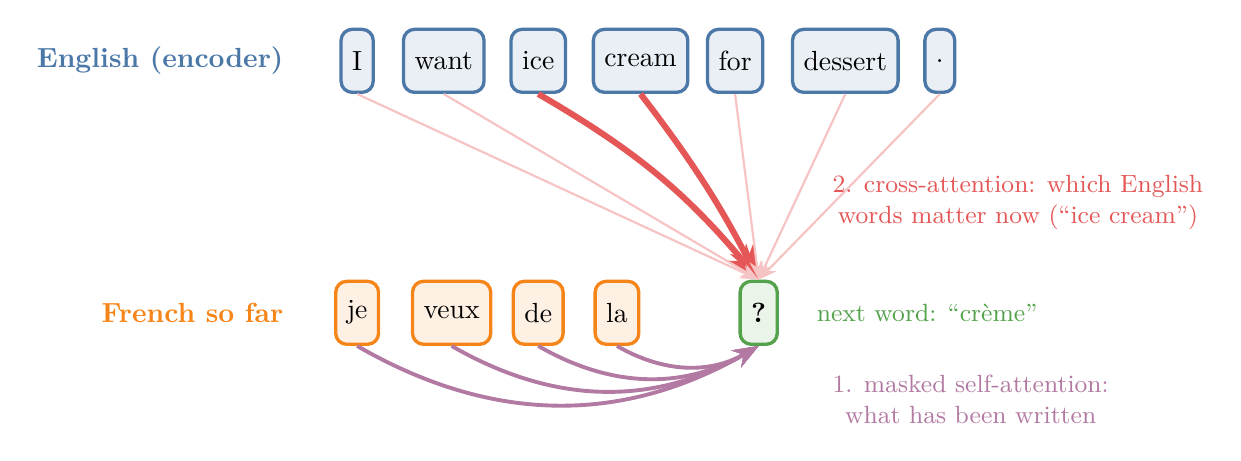
\begin{tikzpicture}[en/.style={box=cblue, inner sep=4pt, minimum height=0.8cm, font=\sffamily},
  fr/.style={box=corange, inner sep=4pt, minimum height=0.8cm, font=\sffamily}]
  \node[anchor=east, font=\sffamily\bfseries, text=cblue] at (-0.5,3.2) {English (encoder)};
  \foreach \w/\x [count=\k] in {I/0.3, want/1.4, ice/2.6, cream/3.9, for/5.1, dessert/6.5, ./7.7} \node[en] (e\k) at (\x,3.2) {\w};
  \node[anchor=east, font=\sffamily\bfseries, text=corange] at (-0.5,0) {French so far};
  \foreach \w/\x [count=\k] in {je/0.3, veux/1.5, de/2.6, la/3.6} \node[fr] (f\k) at (\x,0) {\w};
  \node[box=cgreen, inner sep=4pt, minimum height=0.8cm, font=\sffamily\bfseries] (nx) at (5.4,0) {?};
  \foreach \k in {1,2,3,4} \draw[cpurple, line width=1.4pt, -{Stealth}] (f\k.south) to[bend right=30] (nx.south);
  \node[note, text=cpurple, anchor=west] at (6.2,-1.1) {1. masked self-attention:\\what has been written};
  \draw[cred, line width=2.2pt, -{Stealth}] (e3.south) to[bend left=10] (nx.north);
  \draw[cred, line width=2.2pt, -{Stealth}] (e4.south) to[bend left=5] (nx.north);
  \foreach \k in {1,2,5,6,7} \draw[cred!35, line width=0.8pt, -{Stealth}] (e\k.south) -- (nx.north);
  \node[note, text=cred, anchor=west] at (6.2,1.4) {2. cross-attention: which English\\words matter now (``ice cream'')};
  \node[note, text=cgreen, anchor=west] at (6.0,0) {next word: ``crème''};
\end{tikzpicture}
\end{document}
